%!TEX root = ../../thesis.tex
\chapter{Phage Mosaicism}
\label{ch:phage}

\section{Introduction}
\label{phage:introduction}

Phages are microbial viruses which can infect bacteria, archaea, or single-celled eukaryotes.
By some measures, they are the most abundant and diverse class of organism on the planet.
It is estimated that there are $10^{31}$ extant bacteriophages \cite{Rohwer:2014vz}.\footnote{The estimate can be arrived at two independent ways: by assuming a total bacterial population size of $10^{30}$, and approximately ten phages per bacteria; or by the observation of a phage density of $10^{6}$ to $10^{7}$ per mL of seawater.}
The phage population completely turns over every few days -- an estimated infection rate of $10^{23}$ per second \cite{Suttle:2007cj}.

Phages play an essential role in natural ecosystems by regulating bacterial populations.
Steps have been taken towards harnessing this ability for productive use -- the FDA has approved several bacteriophage products designed to kill harmful bacteria in dairy and meat products \cite{Bren:2007wn}.
Also promising are potential phage therapies for treating pathogenic bacterial infections, although research in this direction is controversial \cite{Keen:2012du}.

Phages are classified based on lifestyle: virulent phages have a lytic life cycle and will infect a host, multiply, and exit the cell via lysis, killing the host organism; temperate phages have a lysogenic life cycle and can remain within the host in a latent state, without disrupting host cellular function.
Phages can have a nucleic acid composition that is either double-stranded DNA (dsDNA), single-stranded DNA (ssDNA), double-stranded RNA (dsRNA), or single-stranded RNA (ssRNA).
Of these, dsDNA is by far the most common.
The typical phage genome length is on the order of $10^{5}$ bases, but can range from $10^{3}$ to $10^{6}$ bases.

Because there is no conserved gene across all phage populations, there is no accepted way of constructing a molecular phage taxonomy.
The current bacteriophage taxonomy is compiled by the International Committee on Taxonomy of Viruses (ICTV) and is based on virus morphology, host range, lifestyle, and nucleic acid composition \cite{ICTV:2012}.
Table~\ref{phage:table:families} presents an overview of phage families as defined by the ICTV.
There are two assigned orders and eighteen recognized families.
Fourteen families have dsDNA, two families have ssDNA, and two families have an RNA genome.

% phage:table:families
\begin{table}[t]
    \caption{Phage families defined by the ICTV}
    \centering
    \scriptsize
    \begin{tabularx}{\textwidth}{lXlX}
    \toprule
    Order & Family & Morphology & Nucleic acid \\
    \midrule
    \multirow{3}{*}{\emph{Caudovirales}} & \emph{Myoviridae}   & Nonenveloped, contractile tail           & linear dsDNA \\
                                         & \emph{Siphoviridae} & Nonenveloped, noncontractile tail (long) & linear dsDNA \\
                                         & \emph{Podoviridae}  & Nonenveloped, noncontractile tail (short) & linear dsDNA \\
    \midrule
    \multirow{2}{*}{\emph{Ligamenvirales}} & \emph{Lipothrixviridae} & Enveloped, rod-shaped    & linear dsDNA \\
                                           & \emph{Rudiviridae}      & Nonenveloped, rod-shaped & linear dsDNA \\
    \midrule
    \multirow{13}{*}{Unassigned} & \emph{Ampullaviridae} & Enveloped, bottle-shaped   & linear dsDNA\\
                                 & \emph{Bicaudaviridae} & Nonenveloped, lemon-shaped & circular dsDNA \\
                                 & \emph{Clavaviridae}   & Nonenveloped, rod-shaped   & circular dsDNA \\
                                 & \emph{Corticoviridae} & Nonenveloped, isometric    & circular dsDNA \\
                                 & \emph{Cystoviridae}   & Enveloped, spherical       & segmented dsRNA \\
                                 & \emph{Fuselloviridae} & Nonenveloped, lemon-shaped & circular dsDNA \\
                                 & \emph{Globuloviridae} & Enveloped, isometric       & linear dsDNA \\
                                 & \emph{Guttaviridae}   & Nonenveloped, ovoid        & circular dsDNA \\
                                 & \emph{Inoviridae}     & Nonenveloped, filamentous  & circular ssDNA \\
                                 & \emph{Leviviridae}    & Nonenveloped, isometric    & linear ssRNA \\
                                 & \emph{Microviridae}   & Nonenveloped, isometric    & circular ssDNA \\
                                 & \emph{Plasmaviridae}  & Enveloped, pleomorph       & circular dsDNA \\
                                 & \emph{Tectiviridae}   & Nonenveloped, isometric    & linear dsDNA \\
    \bottomrule
    \end{tabularx}
    \label{phage:table:families}
\end{table}

Phages have been shown to be subject to high rates of reticulate genomic exchange \cite{Westmoreland:1969dd}.
The phage genome was believed to be mosaic, composed of distinct modules that can be freely exchanged within a population.
Increased genomic data has confirmed this mosaic structure and raised questions about the applicability and interpretation of the ICTV taxonomy.
Based solely on morphology and host, the ICTV taxonomy has been shown to be inconsistent with the genomic data, as the following example from Lawrence \emph{et al.} shows \cite{Lawrence:2002eg}.
In Figure~\ref{phage:fig:inconsistency} we show three different bacteriophage species: Enterobacteria phage HK97, Mycobacterium phage L5, and Enterobacteria phage P22.
HK97 is a Siphoviridae infecting \emph{E. coli}.
L5 is a Siphoviridae infecting \emph{M. smegmatis}.
P22 is a Podoviridae infecting \emph{S. enterica}.
HK97 and L5 belong to the Siphoviridae family comprised of long tail noncontractile phages.
P22 belongs to the Podoviridae family comprised of short tail phages.
Visually, it appears that HK97 and L5 should indeed be classified as distinct from P22.
However, genomic analysis reveals that HK97 and L5 share no gene content, and, despite appearances to the contrary, HK97 and P22 share 20\% gene content.
This example demonstrates that morphology and host range alone are not sufficient in representing phage relationships.

\begin{figure}
\centering
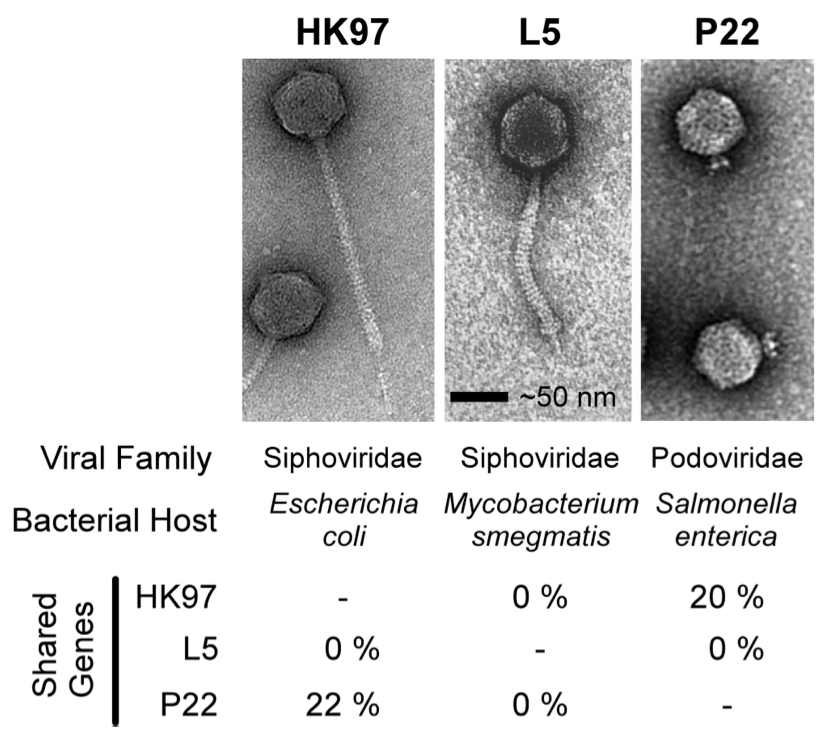
\includegraphics[width=.5\linewidth]{./fig/phage/LAWRENCE_phage_comparative.png}
\caption[Inconsistency of morphological classifications in bacteriophage]{Inconsistency of morphological classifications in bacteriophage. HK97 and L5 are classified in the Siphoviridae family of long tail non-contractile phages, despite sharing no gene content. P22, a short-tail phage in the Podoviridae family, while morphologically dissimilar, shares 20\% gene content with HK97. Figure adapted from \parencite{Lawrence:2002eg}.}
\label{phage:fig:inconsistency}
\end{figure}

Alternative representations of phage relationships have been proposed based on whole genome analysis.
For example, Rohwer and Edwards constructed a phage phylogenetic tree using differences in phage proteomes \cite{Rohwer:2002uo}.
Proux \emph{et al.} proposed a phylogenetic representation based on comparative analysis of head and tail sequences \cite{Proux:2002gj}.
However, these models still make the assumption of tree-like relationships, which will not be appropriate for representing highly mosaic molecular relationships.

In this chapter, we use approaches from topological data analysis to identify, measure, and represent reticulate evolution in a population of phage sequences.
This work is primarily based on data collected by Lima-Mendez \emph{et al.} \cite{LimaMendez:2008ki}.
First, we use persistent homology to characterize reticulation in phage genomes.
We find $H_0$ is largely inconsistent with existing phage taxonomies, and interpret $H_1$ as evidence for reticulate genetic exchange due to shared ecology and host range.
Second, we visualize phage molecular relationships using Mapper, identifying clusters of phages with common gene content and host range.
Representative protein families for each phage cluster are identified.
The Mapper network suggests an alternate way of representing phage molecular relationships.

\section{Data}

We use data initially collected an analyzed in \cite{LimaMendez:2008ki}.
The initial data set consists of a collection of 306 sequenced bacteriophage genomes.
We show summary information about the data in Figure~\ref{phage:fig:phage_data_plot}.
Of the 306 genomes, 246 consist of dsDNA, 36 ssDNA, 12 dsRNA, and 8 ssRNA.
Four have unclassified nucleic acid material.
With respect to lifestyle, 146 are temperate and 72 are virulent.
Actinoplanes phage phiAsp2 is the single pseudotemperate phage, which means it largely maintains a temperate lifestyle but can occasionally enter a virulent state.
For 87 phages the lifestyle is unknown.
Taxonomically, the vast majority belong to order Caudovirales (221), which comprises Siphoviridae (117), Myoviridae (47), and Podoviridae (54). 
Order Ligamenviralies (4) comprises Lipothrixviriae (2) and Rudiviridae (2).
Unassigned families include Inoviridae (22), Cystoviridae (12), Gokushoviridae (8), and Microviridae (6).

\begin{figure}
\centering
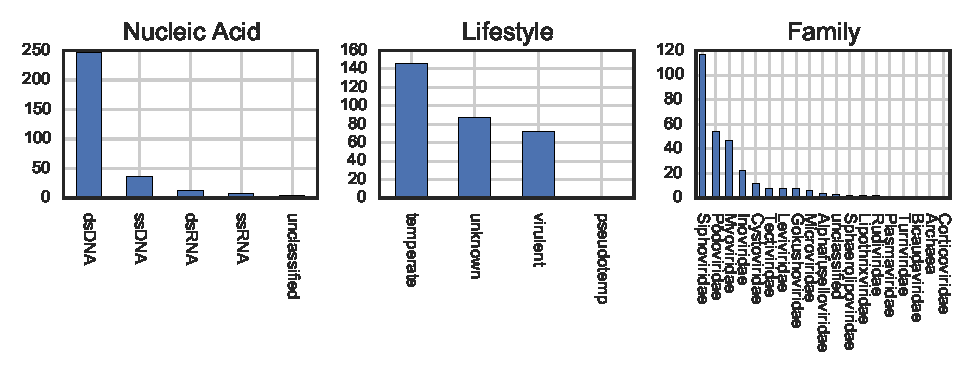
\includegraphics[]{./fig/phage/phage_data_plots.pdf}
\caption[Summary annotations of 306 bacteriophage strains used in this study]{Summary annotations of phage data used in this analysis. 306 bacteriophage genomes were included, as originally collected in \cite{LimaMendez:2008ki}. Here we show various annotations for the phage, including nucleic acid type, lifestyle, and taxonomic family (as defined by the ICTV). For some phage strains this data is unknown.}
\label{phage:fig:phage_data_plot}
\end{figure}

Each of the 306 bacteriophage genomes has been sequenced and annotated.\footnote{The annotation step assigns genes to subsequences of the genome. For well-characterized species this is facilitated by a reference genome. For less well-characterized species this can require the use of heuristic gene-finding algorithms.}
This step resulted in 19,537 unique bacteriophage phage genes.
In the original study \cite{LimaMendez:2008ki}, these genes were then clustered into 8,576 protein families using BlastP, which analyzes pairwise similarity of proteins \cite{Altschul:1997a}.
Protein families share homology, which implies some degree of shared evolutionary ancestry.
Phages can then be represented as phyletic profiles in a protein family-space, indicating the presence or absence of a particular protein family.
In this case, the phyletic matrix $P$ is a $306\times8576$ binary matrix.

\section{Measuring Phage Mosaicism with Persistent Homology}
\label{phage:ph}

We apply persistent homology to the phyletic profiles in order to quantify reticulation in the bacteriphage data.
Because we have transformed from sequence space into phyletic profiles, we do not invoke a specific evolutionary model.
However, the fundamental theorem that non-trivial homology implies reticulation still holds.
First, we construct an appropriate metric space.
Following \cite{LimaMendez:2008ki}, we use a hypergeometric model as follows.
For two phages $A$ and $B$, let $a$ be the number of protein families in phage $A$, $b$ be the number of protein families in phage $B$, and $c$ be the number of protein families in common.
Let $n$ be the total number of protein families.
Then we can compute the p-value that the number of shared protein families $c$ is significant as
\begin{equation}
P_{AB} = \sum_{i=c}^{\min(a,b)} \frac{\binom{a}{i}\binom{n-a}{b-i}}{\binom{n}{b}}.
\end{equation}
To convert the p-values into a distance we take the log transform with small added noise,
\begin{equation}
d_{AB} = \log_{10}(P_{AB} + 10^{-10}) + 10.
\end{equation}
This yields a distance matrix $D$ with distances scaled between $0$ and $10$.
While this space does not explicitly reflect evolutionary divergence at a molecular level, it may be realistic at the protein level at which more complex types of genome evolution will have occurred.

We now compute the persistent homology of $D$.
The barcode diagram is shown in Figure~\ref{phage:fig:barcode}.
The $H_0$ information represents hierarchical clustering and can be identically represented as a dendrogram.
We show the dendrogram, restricting only to strains of order Caudovirales, in Figure~\ref{phage:fig:caudosubset_dendrogram}.
The strains are labeled by their taxonomic family: red for Myoviridae, blue for Siphoviridae, and green for Podoviridae.
We can immediately see that the assigned taxonomic families are not consistent with the clustering based on protein information.
However, there does appear to be some structure in which the taxonomic label is consistent within clusters of strains.
Returning to the barcode diagram, we see substantial nontrivial homology in $H_1$ across all scales.
This confirms the presence of mosaic exchange expected in phage genomes.
% Cycles in $H_1$ can be mapped to specific reticulation patterns. (include???)

\begin{figure}
\centering
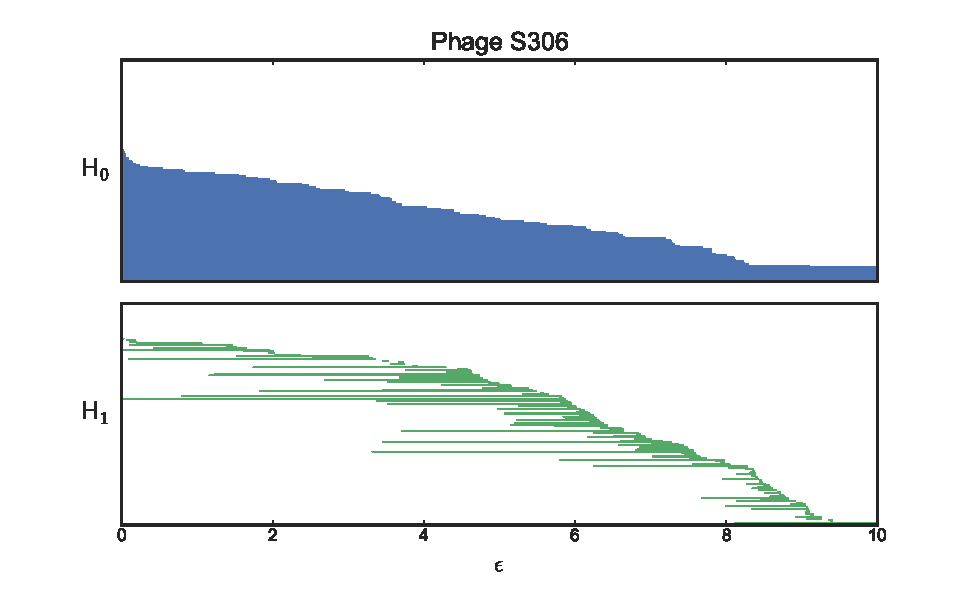
\includegraphics[]{./fig/phage/phage_s306_barcode.pdf}
\caption[S306 Bacteriophage Barcode Diagram]{Bacteriophage Barcode Diagram using the S306 dataset}
\label{phage:fig:barcode}
\end{figure}

\begin{figure}
\centering
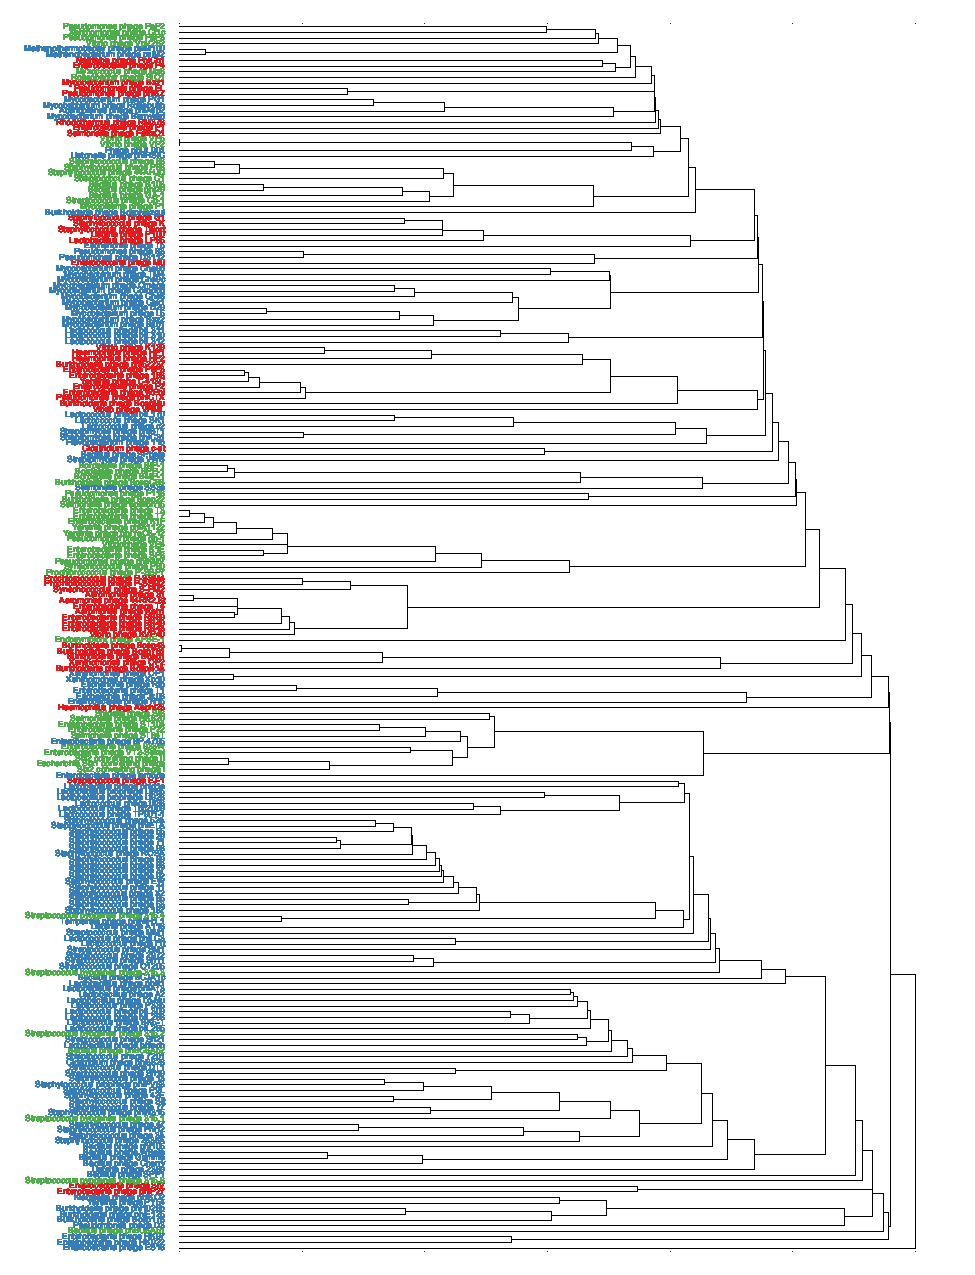
\includegraphics[width=.9\textwidth]{fig/phage/phage_s306_caudosubset_dendrogram.pdf}
\caption[Caudovirales $H_0$ dendrogram]{The dendrogram constructed from the $H_0$, restricted to bacteriophages of order Caudovirales. Myoviridae in red, Siphoviridae in blue, and Podoviridae in green. The family classifications are inconsistent with the hierarchical clustering.}
\label{phage:fig:caudosubset_dendrogram}
\end{figure}

Focusing on order Caudovirales, for which the most data was present.
We separately computed persistent homology for each of the three families.
The barcode diagrams are shown in Figure~\ref{phage:fig:caudovirales_barcodes}.
Computing the TOP score for each family, we have Myoviridae = 0.58, Siphoviridae = 1.14, and Podoviridae = 0.56.

\begin{figure}
\centering
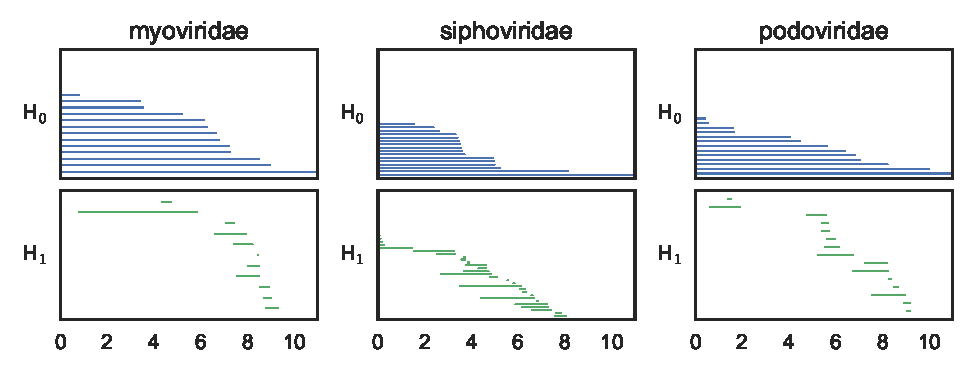
\includegraphics[]{fig/phage/phage_s306_caudovirales_barcodes.pdf}
\caption[Caudovirales Barcode Diagrams]{Barcode Diagrams for Families of Order Caudovirales, including Siphoviridae, Myoviridae, and Podoviridae.}
\label{phage:fig:caudovirales_barcodes}
\end{figure}

\section{Representing Phage Relationships with Mapper}
\label{phage:mapper}

We used Ayasdi Mapper to construct a network representation of the phage phyletic profiles.
The network was constructed using a Hamming metric on the phyletic matrix and a 2D filter function.
The first filter was Metric PCA coordinate 1 with a resolution of 20 and a gain of 3.\footnote{The parameter settings are in arbitrary units and tuned by hand to produce the most visually useful graph.}
The second filter was Metric PCA coordinate 2 with a resolution of 20 and a gain of 3.
The equalize setting was used for both filter functions, which ensures that in the filtered space each bin has approximately the same number of points.
This resulted in a network consisting of 201 nodes from the original 306 rows.
The basic structure of the network is shown in Figure~\ref{phage:fig:phage_mapper_network}, where node color corresponds to the number of phages contained in the node.
The network consists of one large connected component, two smaller connected components, and 21 singly connected nodes.
The large connected component has local regions of clustering, which will be considered further later.

\begin{figure}
\centering
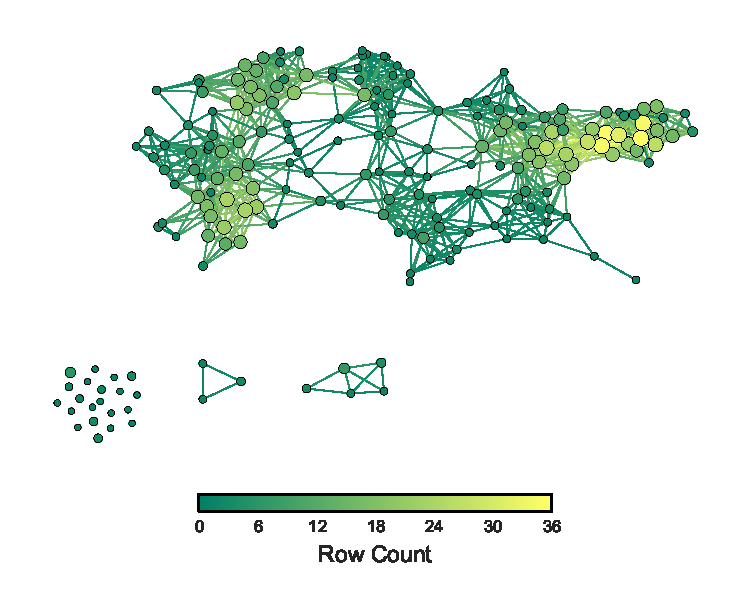
\includegraphics[]{{fig/phage/phage.s306.mapper_network}.pdf}
\caption[Phage Mapper Network]{Phage Mapper Network. Network constructed using Mapper as implemented in Ayasdi Iris \cite{AyasdiIris:2015}. The network was constructed using a Hamming metric with a 2D Metric PCA filter function (resolution=20, gain=3, equalize). Nodes in the network represent clusters of phages and edges connect nodes that contain samples in common. Nodes are colored by the number of phages in each node.}
\label{phage:fig:phage_mapper_network}
\end{figure}

We first examined how well the existing taxonomic classifications localized in the Mapper representation.
If the taxonomy accurately reflects the molecular characteristics that were used to construct the network, we would expect to see strains belonging to the same level of hierarchy as localized together in the network, with minimal mixing between strains of different classification.
We show the representation of the three families of order Caudovirales in Figure~\ref{phage:fig:s306_caudovirales_networks}.
Each node is colored by the proportion of rows from that family contained in the node.\footnote{Recall that the nodes in a Mapper network can be composed of multiple nodes, depending on the parameters of the filter function used.}
We immediately see that each family is widely dispersed across the network.
On closer examination, we see that the patterns of spread resemble those of the dendrogram in Figure~\ref{phage:fig:caudosubset_dendrogram}, in that there are multiple clusters core clusters for each family.
For example, the Myoviridae family has clusters in the bottom left and bottom right of the large component, and two singleton clusters.
This roughly corresponds to the four clusters of Myoviridae in the $H_0$ dendrogram.

How strongly a particular classification is reflected by a network can be quantitatively measured using a modularity score \cite{Newman:2006iq}.
Modularity was originally devised for identifying community structure in networks.
Intuitively, more tightly localized network divisions will have a higher modularity, while dispersed divisions will have a lower modularity.
The standard definition for a two-class division is
We use a modified form of modularity 
\begin{equation}
Q = \frac{1}{m}\sum_{ij} A_{ij}s_{i}s_{j}
\end{equation}
where $m$ is the total number of edges in the network, $A$ is the adjacency matrix of the network, and $s_{i}=\pm1$ is the class membership of node $i$.\footnote{The standard definition of modularity includes a term measuring how tightly connected each module is.We are only interested in the localization of each modular and neglect this term.}
The modularity ranges between $0$ and $1$.
We use a strict class membership, in which $s_{i}=1$ for node $i$ if any row in the now contains the annotation of interest.
The modularity score for each family of Caudiovirales is shown in Figure~\ref{phage:fig:s306_mapper_modularities}.

\begin{figure}
\centering
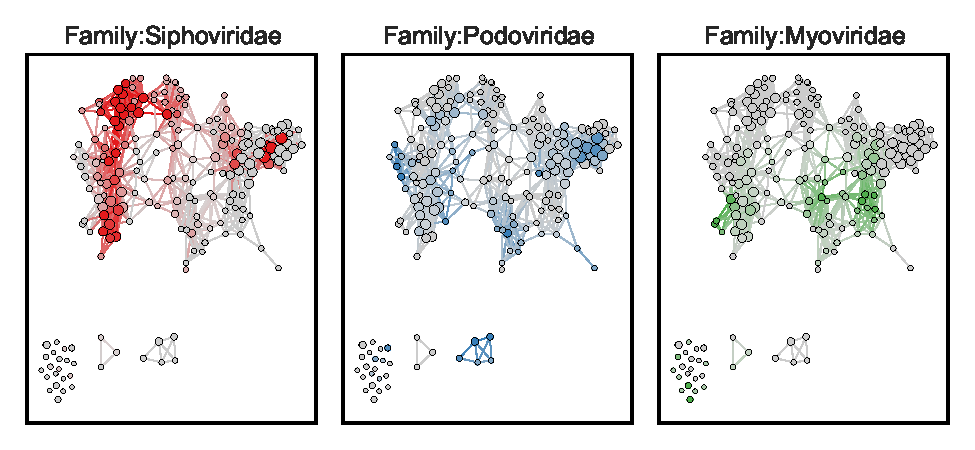
\includegraphics[]{{fig/phage/phage.s306.caudovirales_networks}.pdf}
\caption[Phage Network Colored by Taxonomic Family]{Taxonomic localization in the bacteriophage network. Network nodes are colored by presence of phages for each family in order Caudovirales.}
\label{phage:fig:s306_caudovirales_networks}
\end{figure}

\begin{figure}
\centering
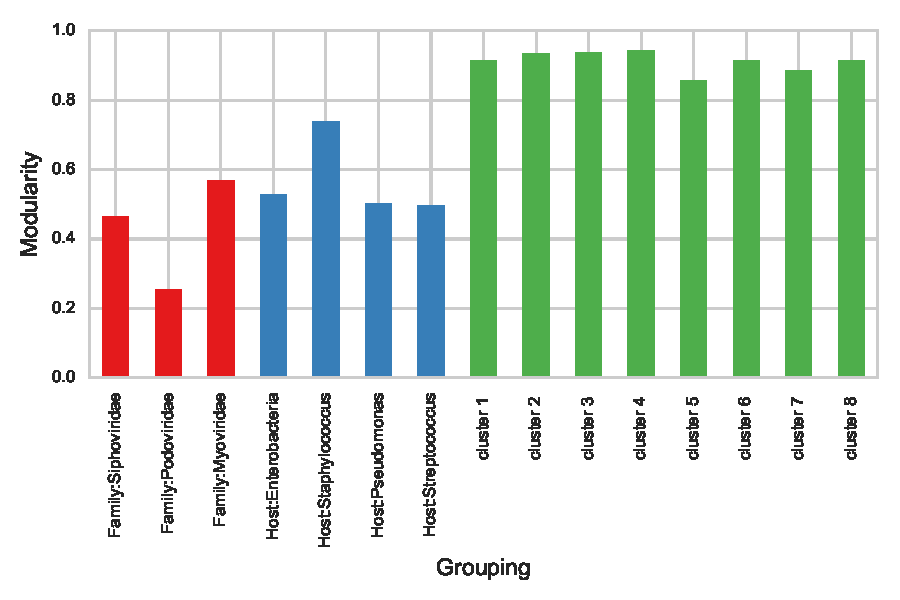
\includegraphics[]{fig/phage/phage_s306_mapper_modularities.pdf}
\caption[Modularity Scores for Different Divisions of the Phage Network]{Modularity Scores for Different Divisions of the Phage Network. We show the modularities for divisions defined by taxonomic family and host range, as well as the clusters we identify using MCL.}
\label{phage:fig:s306_mapper_modularities}
\end{figure}

Second, we examined how well host correlated with network structure.
We show this for the top six hosts represented in our dataset in Figure~\ref{phage:fig:s306_host_networks}.
While Enterobacteria has several pockets of representation within the network, phages are on average more strongly clustered by host than by taxonomy.
This is consist with existing evidence that phages of similar host range have a common environment for reticulate exchange\cite{Lawrence:2002eg}.
Modularity scores for the most dominant four hosts are shown in Figure~\ref{phage:fig:s306_mapper_modularities}.
Staphylococcus has the highest defined modularity, which is consistent with the earlier reports about strong coupling and high levels of exchange between the Staphylococcus host and its viruses \cite{Deghorain:2012wv}.

\begin{figure}
\centering
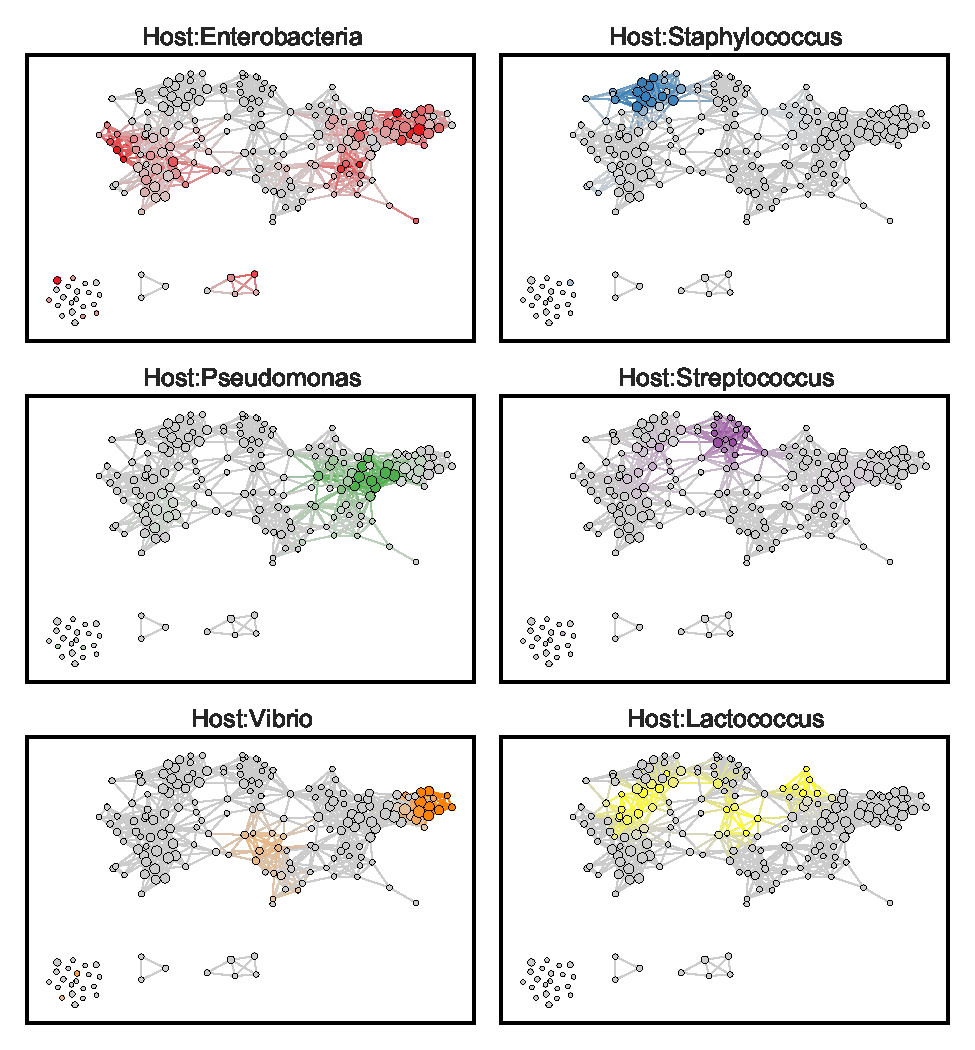
\includegraphics[]{{fig/phage/phage.s306.host_networks}.pdf}
\caption[Phage Network Colored by Host]{Host localization in the bacteriophage network. Compared to taxonomic family, phages are more tightly localized, reflecting the degree to which shared host range provides an environment for reticulate exchange.}
\label{phage:fig:s306_host_networks}
\end{figure}

Finally, we clustered the network using the MCL graph clustering algorithm \cite{Enright:2002ep}, as implemented in the Python MCLMarkovCluster package \cite{Lami:2014}.
The MCL algorithm takes two input parameters which control the coarseness of the clustering: an expansion factor $e$ and an inflation factor $i$.
We set $e=5$ and $i=5$.
Ignoring the singleton nodes, this resulted in eleven clusters, as shown in Figure~\ref{phage:fig:s306_mcl_clustered_network}.
For each cluster, we used a hypergeometric test to identify particular protein families that were over- or under-represented in each cluster.
After correcting for multiple testing, the protein families were most significantly associated with particular clusters are shown in Table~\ref{phage:table:cluster_functions}.

\begin{figure}
\centering
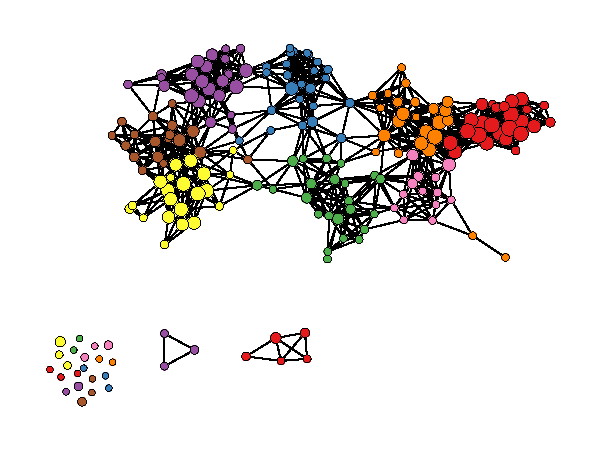
\includegraphics[]{{fig/phage/phage.s306.mcl_clustered_network}.pdf}
\caption[Phage Network with MCL Clustering]{Phage Network with MCL Clustering. 11 nontrivial clusters are identified. In Table~\ref{phage:table:cluster_functions} we associate clusters with representative protein families.}
\label{phage:fig:s306_mcl_clustered_network}
\end{figure}

% phage function table.
\begin{sidewaystable}
    \caption{Phage Network MCL clustering annotations and representative protein families}
    \tiny

    % define tables
    \begin{lrbox}{\leftbox}
            \begin{tabular}[t]{llll}
            \toprule
            Cluster & Protein Family & p-value & Function \\
            \midrule
            \multirow{1}{*}{Cluster 1} & pf\_0001 & 6.17e-25 & tail tape measure protein \\ 
                                        & pf\_0002 & 6.81e-21 & transcriptional repressor \\ 
                                        & pf\_0003 & 2.69e-16 & tyrosine based integrase \\ 
                                        & pf\_0004 & 9.08e-12 & DNA binding protein \\ 
                                        & pf\_0008 & 7.37e-10 & unknown \\ 
                                        & pf\_0010 & 2.36e-08 & terminase large subunit \\ 
                                        & pf\_0006 & 2.87e-08 & NA \\ 
                                        & pf\_0164 & 5.57e-08 & NA \\ 
                                        & pf\_0012 & 1.74e-07 & DNA replication inititation protein \\ 
                                        & pf\_0015 & 2.42e-07 & scaffolding protein \\ 
                                        & pf\_0187 & 2.70e-07 & NA \\ 
                                        & pf\_0217 & 2.70e-07 & NA \\ 
                                        & pf\_0013 & 3.35e-07 & NA \\ 
                                        & pf\_0017 & 4.63e-07 & portal protein \\ 
                                        & pf\_0007 & 8.84e-07 & endolysin \\ 
            \midrule
            \multirow{1}{*}{Cluster 2} & pf\_0131 & 9.38e-13 & NA \\ 
                                        & pf\_0279 & 2.33e-09 & NA \\ 
                                        & pf\_0109 & 1.02e-08 & NA \\ 
                                        & pf\_0434 & 4.38e-08 & NA \\ 
                                        & pf\_0435 & 4.38e-08 & NA \\ 
                                        & pf\_0436 & 4.38e-08 & NA \\ 
                                        & pf\_0010 & 1.84e-07 & terminase large subunit \\ 
                                        & pf\_0029 & 2.02e-07 & major head protein \\ 
                                        & pf\_0009 & 2.54e-07 & NA \\ 
                                        & pf\_0093 & 4.61e-07 & NA \\ 
                                        & pf\_0512 & 5.47e-07 & NA \\ 
                                        & pf\_0017 & 7.12e-07 & portal protein \\ 
            \midrule
            Cluster 3 & & & \\
            \midrule
            \multirow{1}{*}{Cluster 4} & pf\_0049 & 3.44e-24 & unknown \\ 
                                        & pf\_0043 & 3.44e-24 & unknown \\ 
                                        & pf\_0053 & 3.86e-23 & unknown \\ 
                                        & pf\_0052 & 3.86e-23 & unknown \\ 
                                        & pf\_0007 & 6.19e-22 & endolysin \\ 
                                        & pf\_0058 & 4.39e-21 & unknown \\ 
                                        & pf\_0060 & 4.39e-21 & unknown \\ 
                                        & pf\_0061 & 4.39e-21 & unknown \\ 
                                        & pf\_0002 & 2.23e-20 & transcriptional repressor \\ 
                                        & pf\_0067 & 4.46e-20 & unknown \\ 
                                        & pf\_0063 & 4.46e-20 & unknown \\ 
                                        & pf\_0012 & 1.12e-19 & DNA replication inititation protein \\ 
                                        & pf\_0018 & 2.04e-19 & tail protein \\ 
                                        & pf\_0072 & 4.38e-19 & unknown \\ 
                                        & pf\_0004 & 1.82e-18 & DNA binding protein \\ 
                                        & pf\_0020 & 5.91e-18 & unknown \\ 
                                        & pf\_0087 & 3.86e-17 & unknown \\ 
                                        & pf\_0042 & 5.24e-17 & unknown \\ 
                                        & pf\_0001 & 1.54e-16 & tail tape measure protein \\ 
                                        & pf\_0092 & 3.48e-16 & unknown \\ 
            \midrule
            \end{tabular}
    \end{lrbox}
    \begin{lrbox}{\rightbox}
            \begin{tabular}[t]{llll}
            \toprule
            Cluster & Protein Family & p-value & Function \\
            \midrule
            \multirow{1}{*}{Cluster 5} & pf\_0008 & 7.45e-07 & unknown \\ 
            \midrule
            \multirow{1}{*}{Cluster 6} & pf\_0006 & 2.17e-18 & NA \\ 
                                        & pf\_0057 & 8.74e-10 & unknown \\ 
                                        & pf\_0142 & 3.84e-09 & unknown \\ 
                                        & pf\_0082 & 1.79e-08 & lysis protein \\ 
                                        & pf\_0165 & 2.09e-08 & prohead \\ 
                                        & pf\_0188 & 1.12e-07 & minor tail protein \\ 
                                        & pf\_0190 & 1.12e-07 & tail \\ 
                                        & pf\_0189 & 1.12e-07 & minor tail protein \\ 
                                        & pf\_0204 & 5.81e-07 & unknown \\ 
            \midrule
            \multirow{1}{*}{Cluster 7} & pf\_0002 & 8.92e-11 & transcriptional repressor \\ 
                                        & pf\_0121 & 2.46e-09 & transcription factor  \\ 
                                        & pf\_0016 & 3.36e-08 & unknown \\ 
                                        & pf\_0122 & 6.52e-08 & unknown \\ 
                                        & pf\_0156 & 3.35e-07 & NA \\ 
                                        & pf\_0517 & 4.38e-07 & NA \\ 
                                        & pf\_0004 & 5.26e-07 & DNA binding protein \\ 
                                        & pf\_0135 & 5.97e-07 & unknown \\ 
                                        & pf\_0176 & 9.43e-07 & post-translational regulator \\ 
                                        & pf\_0178 & 9.43e-07 & unknown \\ 
                                        & pf\_0177 & 9.43e-07 & transcription anti-termination protein \\ 
                                        & pf\_0012 & 9.78e-07 & DNA replication inititation protein \\ 
                                        & pf\_0324 & 1.06e-06 & NA \\ 
                                        & pf\_0325 & 1.06e-06 & NA \\ 
            \midrule
            \multirow{1}{*}{Cluster 8} & pf\_0497 & 1.24e-07 & NA \\ 
                                        & pf\_0417 & 8.23e-07 & NA \\ 
                                        & pf\_0002 & 9.70e-07 & transcriptional repressor \\ 
            \midrule
            \multirow{1}{*}{Cluster 9} & pf\_0425 & 2.15e-14 & NA \\ 
                                        & pf\_0424 & 2.15e-14 & NA \\ 
                                        & pf\_0423 & 2.15e-14 & NA \\ 
                                        & pf\_0422 & 2.15e-14 & NA \\ 
                                        & pf\_0421 & 2.15e-14 & NA \\ 
                                        & pf\_0420 & 2.15e-14 & NA \\ 
                                        & pf\_0146 & 2.15e-14 & NA \\ 
                                        & pf\_0366 & 1.72e-13 & NA \\ 
                                        & pf\_0316 & 7.74e-13 & NA \\ 
                                        & pf\_0315 & 7.74e-13 & NA \\ 
                                        & pf\_0273 & 2.58e-12 & NA \\ 
                                        & pf\_0274 & 2.58e-12 & internal virion protein \\ 
                                        & pf\_0138 & 2.58e-12 & head protein \\ 
                                        & pf\_0504 & 6.45e-12 & NA \\ 
                                        & pf\_0503 & 6.45e-12 & NA \\ 
                                        & pf\_0183 & 7.09e-12 & NA \\ 
                                        & pf\_0184 & 1.70e-11 & portal protein \\ 
                                        & pf\_0185 & 1.70e-11 & tail protein \\ 
                                        & pf\_0163 & 1.70e-11 & tail protein \\ 
                                        & pf\_0426 & 4.50e-11 & NA \\ 
            \bottomrule
            \end{tabular}
    \end{lrbox}


    \centering
    \makebox[0pt]{%
        \hspace*{\fill}
        \begin{minipage}[t]{\wd\leftbox}
        \usebox{\leftbox}
        \end{minipage}\hfill
        \begin{minipage}[t]{\wd\rightbox}
        \usebox{\rightbox}
        \end{minipage}
        \hspace*{\fill}
        }
    \label{phage:table:cluster_functions}
\end{sidewaystable}

\section{Conclusions}
\label{phage:sec:conclusions}

In this chapter, we analyzed reticulate evolution in bacteriophages, using data from fully sequenced phage genomes represented as phyletic profiles measuring gene content.
First, we used persistent homology to show that there are high levels of reticulate exchange across multiple taxonomic scales.
Information in the $H_0$ barcode confirmed the inconsistency of the ICTV classification.
Information in the $H_1$ barcode was used to compare levels of reticulate exchange among different phages.
Second, we used Mapper to construct a network representation of phage molecular relationships.
We examined how well different annotations, including taxonomic classification and host range, localized on this network.
We used a network clustering algorithm to identify communities of phages related by shared protein content, and identified protein families representative of each cluster.
These clusters, while not explicitly reflecting potential phylogenetic trajectories, are more reflective of molecular similarity than existing morphological taxonomies, and can be used as a starting point for developing a more comprehensive picture of bacteriophage evolutionary dynamics.
Further sequencing data will allows us to refine these clusters and provide a higher resolution 
